\documentclass[11pt]{article}
\usepackage{homework}

\classname{361}
\homeworknum{0}



\begin{document}

% Environments

\newcommand{\state}[2]{\begin{statement}{#1} #2 \end{statement}}
\newcommand{\prob}[2]{\begin{problem}{#1} #2 \end{problem}}
\newcommand{\subprob}[1]{\begin{subproblem} #1 \end{subproblem}}
\newcommand{\sol}[1]{\begin{solution} #1 \end{solution}}
\newcommand{\fig}[2]{\begin{figure} \centering #2  \label{#1} \end{figure}}

\newcommand{\makebib}{
	\vfill
	\color{black}
	\nocite{*}
	\bibliography{references}{}
	\bibliographystyle{lucas_unsrt}
}
	

% Implication

\newcommand{\qwhere}{\quad \text{where} \quad}
\newcommand{\qimplies}{\quad \implies \quad}
\newcommand{\impliesq}{\implies \quad}



% Brackets

\newcommand{\paren}[1]{\left( #1 \right)}
\newcommand{\brac}[1]{\left[ #1 \right]}
\newcommand{\curly}[1]{\left\{ #1 \right\}}


% Greek

\newcommand{\alp}{\alpha}
\newcommand{\bet}{\beta}
\newcommand{\gam}{\gamma}
\newcommand{\del}{\delta}
\newcommand{\eps}{\epsilon}
\newcommand{\zet}{\zeta}
\newcommand{\tht}{\theta}
\newcommand{\kap}{\kappa}
\newcommand{\lam}{\lambda}
\newcommand{\sig}{\sigma}
\newcommand{\ups}{\upsilon}
\newcommand{\omg}{\omega}

\newcommand{\Gam}{\Gamma}
\newcommand{\Del}{\Delta}
\newcommand{\Tht}{\Theta}
\newcommand{\Lam}{\Lambda}
\newcommand{\Sig}{\Sigma}
\newcommand{\Omg}{\Omega}


% Text

\newcommand{\where}{\text{where }}

% Problem 1

\newcommand{\Hint}{H_\text{int}}
\newcommand{\ddcx}{\dd[3]{x}}
\newcommand{\psib}{\bar{\psi}}

\newcommand{\mh}{m_h}
\newcommand{\mmu}{m_\mu}
\newcommand{\me}{m_e}
\newcommand{\ma}{m_a}

\newcommand{\aexpt}{a_\text{expt.}}
\newcommand{\aQED}{a_\text{QED}}
\renewcommand{\GeV}{\giga\electronvolt}

\newcommand{\gamt}{\gam^5}

\state{}{
	The material $\LaSrCuO$ has a layered crystal structure that consists of two-dimensional square lattices of $\CuO$ planes (shown in Fig.~\ref{f1}) separated by layers of $\LaSrO$.  You may assume that $\La$ has valence $3+$, $\Sr$ valence $2+$, and $\Ox$ valence $2-$; the electrons from these cations are donated uniformly to the widely separated $\CuO$ layers, which thus have a two-dimensional electronic structure.  Neutral atomic $\Cu$ has the configuration $[\Ar] 4s^2 3d^9$.  In this compound, four of the $\Cu$ $d$ levels are completely filled, and there is a partially filled band formed from $d_{x^2 - y^2}$ orbitals.  You may assume the $\Cu$ $4s$ levels are unoccupied, and the $\Ox$ $2p$ levels are fully occupied.  Electronic dispersion perpendicular to the planes may be neglected.
	
	The band structure in the independent particle approximation is well described by a tight-binding model incorporating a single orbital (per unit cell) of $d_{x^2 - y^2}$ symmetry centered on the $\Cu$ atom, with nonzero Hamiltonian matrix elements $t$ between nearest neighbor orbitals in the $x$ and $y$ directions, and matrix elements $t'$ between second neighbors across the diagonals.
	
	\begin{figure}[b!] \centering
		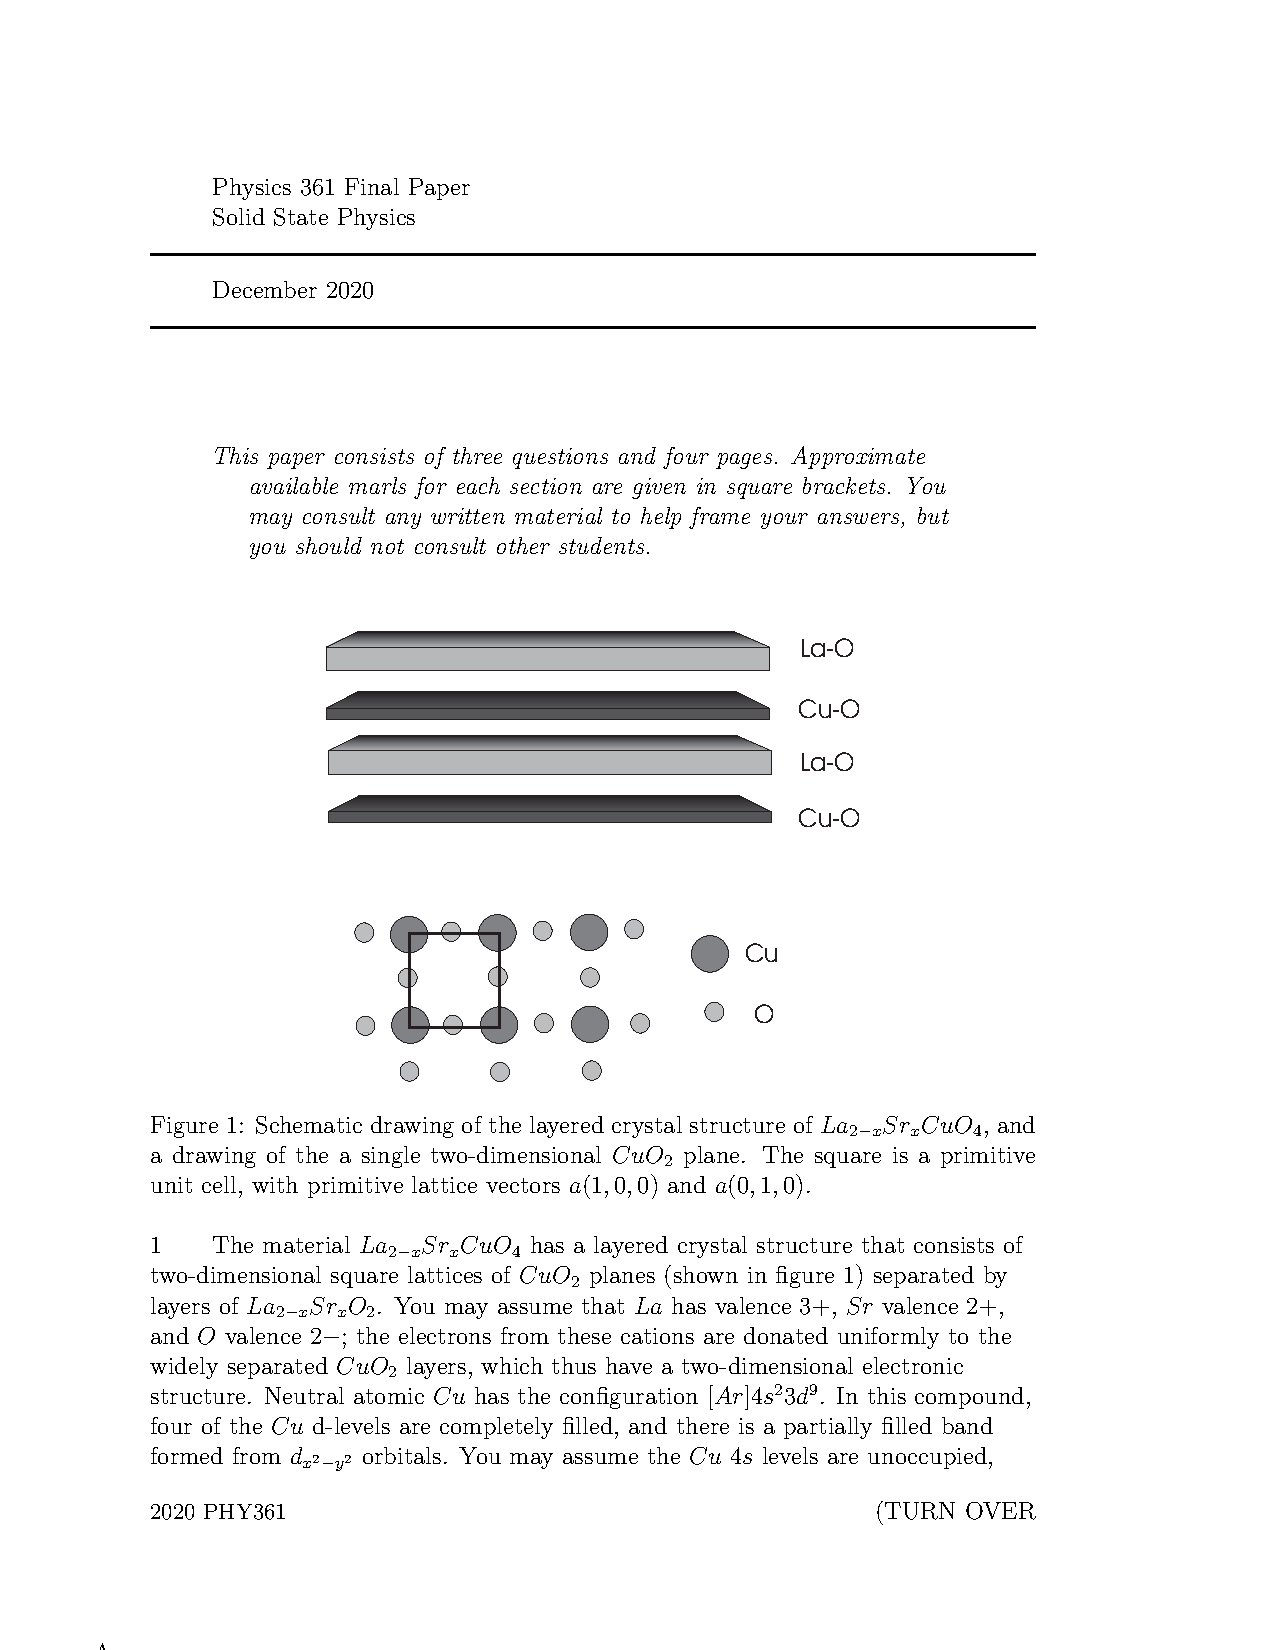
\includegraphics[width=0.5\textwidth,trim=5cm 9.5cm 7cm 10cm,clip]{fig1}
		\caption{Schematic drawing of the layered crystal structure of $\LaSrCuO$, and a drawing of the a single two-dimensional $\CuO$ plane.  The square is a primitive unit cell, with primitive lattice vectors $a(1, 0, 0)$ and $a(0, 1, 0)$.}
		\label{f1}
	\end{figure}
}

\prob{
	Show that in this approximation the energy dispersion of an electron is
	\eq{
		\Ek = 2 t [ \cos(\kx a) + \cos(\ky a) ] + 4 t' \cos(\kx a) \cos(\ky a).
	}
	\vfix
}

\sol{
	The band energy in the tight-binding description is given by (4.57) in the lecture notes,
	\eq{
		\Ek = \epso + t \sumrho e^{-i \vk \vdot \vrho}.
	}
	In the two-dimensional $\CuO$ plane, the four nearest neighbors to the origin are located at
	\eqn{nn}{
		\vrho \in a \{ (1, 0, 0),\ (0, 1, 0),\ (-1, 0, 0),\ (0, -1, 0) \},
	}
	and the four second-nearest neighbors are located at
	\eqn{nnn}{
		\vrho' \in a \{ (1, 1, 0),\ (-1, 1, 0),\ (1, -1, 0),\ (-1, -1, 0) \}.
	}
	So, assuming $\epso = 0$, the band energy is
	\aln{
		\Ek &= t \sumrho e^{-i \vk \vdot \vrho} + t' \sumrhop e^{-i \vk \vdot \vrho'} \notag \\
		&= t \paren{ e^{-i a \kx} + e^{-i a \ky} + e^{i a \kx} + e^{i a \ky} } + t' \paren{ e^{-i a (\kx + \ky)} + e^{i a (\kx - \ky)} + e^{-i a (\kx - \ky)} + e^{i a (\kx + \ky)} } \notag \\
		&= t \paren{ e^{-i a \kx} + e^{i a \kx} + e^{-i a \ky} + e^{i a \ky} } + t' \paren{ e^{-i a \kx} e^{-i a \ky} + e^{i a \kx} e^{-i a \ky} + e^{-i a \kx} e^{i a \ky} + e^{i a \kx} e^{i a \ky} } \notag \\
		&= t \brac{ \paren{ e^{-i a \kx} + e^{i a \kx} } + \paren{ e^{-i a \ky} + e^{i a \ky} } } + t' \paren{ e^{-i a \kx} + e^{i a \kx} } \paren{ e^{-i a \ky} + e^{i a \ky} } \notag \\
		&= t \brac{ 2 \cos(\kx a) + 2 \cos(\ky a) } + t' \brac{ 2 \cos(\kx a) } \brac{ 2 \cos(\ky a) } \notag \\
		&= 2 t [ \cos(\kx a) + \cos(\ky a) ] + 4 t' \cos(\kx a) \cos(\ky a) \label{ans1a}
	}
	as we wanted to show. \qed
}



\prob{ \label{1b}
	What do you expect to be the signs of $t$ and $t'$?  Explain your reasoning.
}

\sol{
	The signs of $t$ and $t'$ are expected to be negative because the Coulomb potential $\Del U$ between the two electrons at any two sites is negative~\cite[pp.~78--79]{Coleman}.  We see that $t$ depends on $\Delta U$ by Ashcroft \& Mermin~(10.18), and we see that $t$ has the same sign as $\Del U$ by (4.56) in the lecture notes:
	\eq{
		t = \int \ddvr \psi^*(\vr - \rho) \Del U \psi(\vr).
	}
	\vfix
}



\prob{
	For the case that $\abs{t' / t} = 0$, sketch the Fermi surface for $\Sr$ concentrations of $x = 0$, $x \approx 0.2$, and $x \approx 0.5$.
}

\sol{
	As $x$ increases, the partially-filled band of $\Cu$ becomes more empty.  When $x = 0$, the band is mostly full.  When $x = 0.5$, it is half full.  Fig.~\ref{f1cd}~(left) shows the Fermi surface in the reduced zone scheme for $x = 0$~(blue line), $x \approx 0.2$~(gold line), and $x \approx 0.5$~(green line) when $t' = 0$~\cite[p.~231]{Kittel}.  The figures were created in Mathematica by plotting Eq.~\refeq{ans1a} and choosing appropriate contours.
}


\begin{figure}[t] \centering
	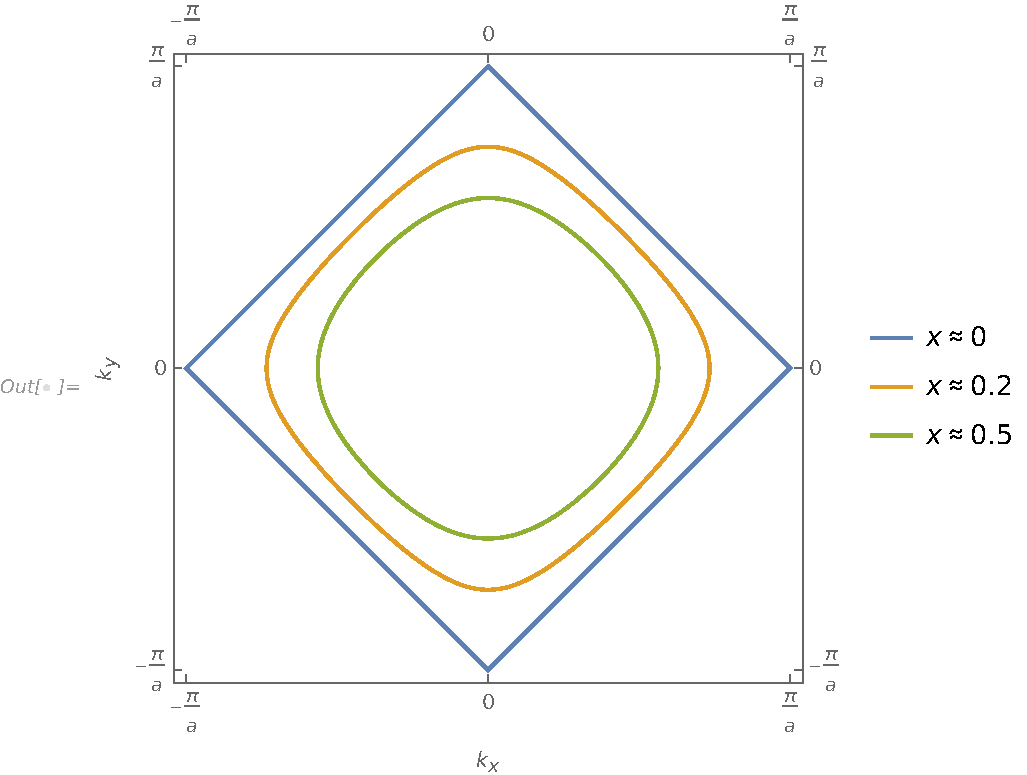
\includegraphics[width=0.49\textwidth,trim=1.5cm 0 0 0,clip]{1c} \hfill
	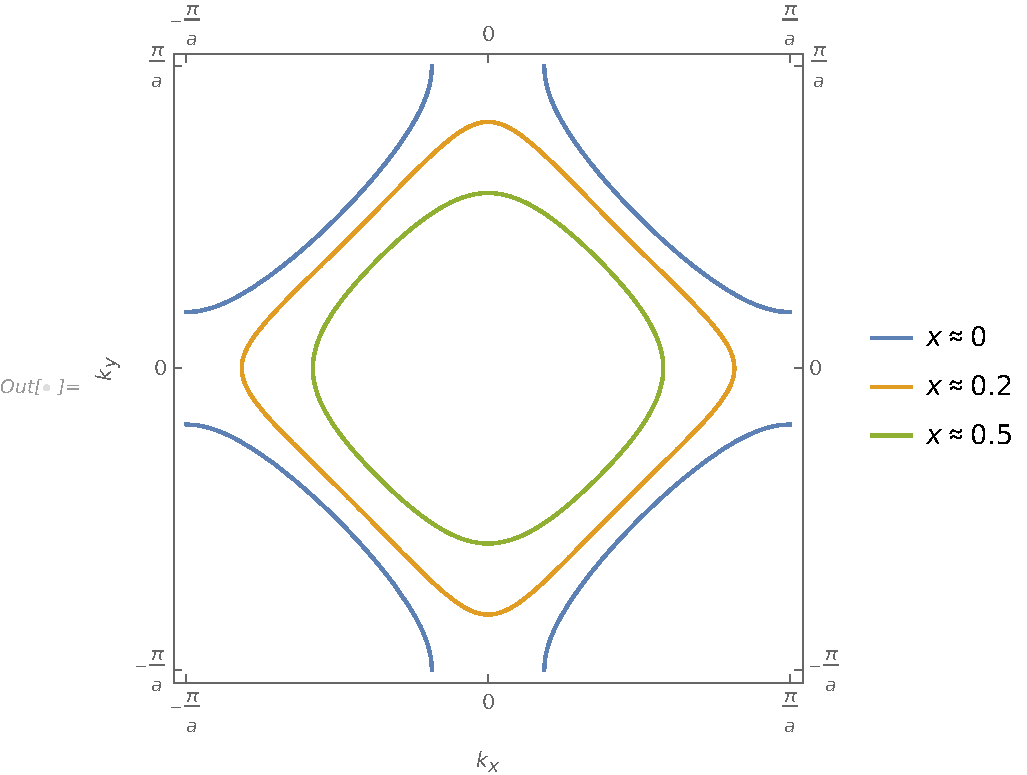
\includegraphics[width=0.49\textwidth,trim=1.5cm 0 0 0,clip]{1d}
	\caption{Fermi surfaces for $t' = 0$~(left) and $\abs{t' / t} = 0.1$~(right) for $x = 0$~(blue line), $x \approx 0.2$~(gold line), and $x \approx 0.5$~(green line).}
	\label{f1cd}
\end{figure}


\prob{ \label{1d}
	How do these contours change qualitatively if $\abs{t' / t} \sim 0.1$?  (Choose the signs of $t$ and $t'$ that you proposed in \ref{1b}.)
}

\sol{
	For $t$ and $t'$ both negative, the contributions from $t'$ will distort the contours by pulling their ends toward the corners of the frame.  This happens because, in general, the Fermi surface is stretched toward the positions of the nearest neighbors (for $t < 0$) given by Eq.~\refeq{nn}.  There is a nearest neighbor at the center of each edge of the frame.  When we also consider $t' < 0$ contributions from the next-nearest neighbors, which are located in the corners of the frame by Eq.~\refeq{nnn}, the Fermi surface is pulled toward those ions as well.  The effect is not too large since $\abs{t'}$ is small compared to $\abs{t}$.  Fig.~\ref{f1cd}~(right) shows the Fermi surface in the reduced zone scheme for $x = 0$~(blue line), $x \approx 0.2$~(gold line), and $x \approx 0.5$~(green line) when $t' = 0.1 t$.
}


\vspace{2in}
\prob{
	Assuming the dispersion of \ref{1d}, sketch the electronic density of states in energy, paying particular attention to the behavior near the edges of the band and at a saddle point in the middle of the band.
}

\sol{
	Our sketch of $\gE$ is based on Fig.~4.2 in the course lecture notes, and is shown in Fig.~\ref{f1e}.  The logarithmic singularity in the middle represents the saddle point.  Near the edges, the curve flattens out.

	\begin{figure}[t] \centering
		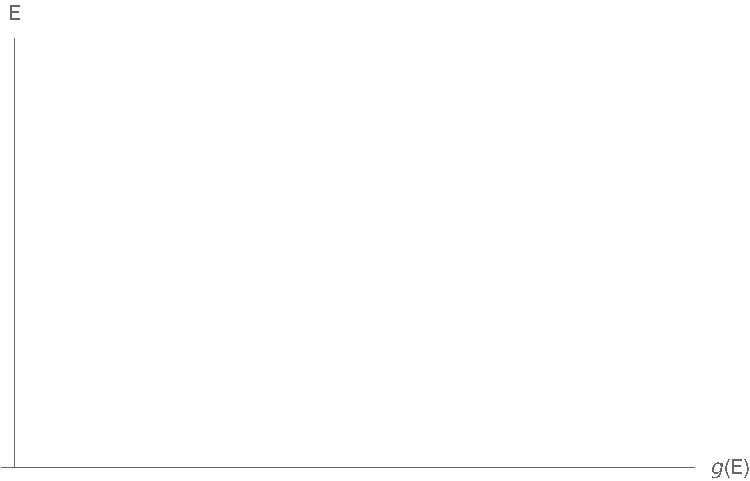
\includegraphics[width=0.5\textwidth]{1e}
		\caption{Density of states $\gE$ for the dispersion shown in Fig.~\ref{f1cd}~(right).}
		\label{f1e}
	\end{figure}
}



\prob{
	What would the independent electron model predict for the temperature dependence of the low-temperature electronic specific heat when the chemical potential is exactly at the saddle point near the middle of the band?
}

\sol{
	By (2.15) in the lecture notes, the electronic specific heat is given by
	\eq{
		\cv = \int \ddE E \gE \dv{\fE}{T},
	}
	where $\fE$ is the Fermi distribution.  At low temperature, the chemical potential is approximately equal to the specific heat.  The saddle points are located at the positions of the nearest neighbors, given by Eq.~\refeq{nn}.  Since the lattice is periodic, we can choose $\vrho = (a, 0, 0)$ without loss of generality.
}



\prob{
	$\LaCuO$ is an antiferromagnetic insulator.  Suggest, and discuss, reason(s) why the ground state differs from that predicted by the band structure in the independent particle approximation.  Your answer should include a qualitative explanation of both the magnetic and the insulating behavior.
}





%\clearpage
%\state{}{ %\hfix 
%(Mathematical results may be stated without proof, and marks will be given for demonstrating a rounded understanding of the topic, for appropriate use of examples, and for good use of figures.  One or two pages of text is expected, in bullet rather than essay form, for each part.)
%}
%
%\prob{
%	Write short notes on the properties of a Fermi liquid.
%}
%
%
%
%\prob{
%	Write short notes on effects due to the electron-phonon interaction in metals.
%}
%
%
%
%\prob{
%	Write short notes on the use of density functional theory to perform practical calculations of ground state properties of solids.
%}
%
%
%
%\prob{
%	Write short notes on photoemission spectroscopy.
%}
%
%
%
%
%
%\clearpage
%\state{}{
%	A long-wavelength optical phonon in an insulating ionic solid is described by the following equation of motion:
%	\eq{
%		M \vudd + K \vuu = Q \vE,
%	}
%	where $\vuu$ is the atomic displacement, $M$ the mass, $K$ a local restoring force, and $\vE$ is the electric field.  A displacement of the ions by $\vuu$ results in a polarization
%	\eq{
%		\vP = n Q \vuu,
%	}
%	where $n$ is the density of the ions, and $Q$ their effective charge.  We will consider only longitudinal modes, where $\vD$, $\vE$, $\vuu$ are all parallel.
%}
%
%\prob{
%	Neglecting any further electronic response of the solid, calculate the response of the phonon mode to a uniform external electric displacement field $\vD = \epso \vE + \vP$, oscillating with a frequency $\omg$.  Hence show that the phonon contribution to the frequency-dependent dielectric function, defined by $D = \epsion \epso E$ may be written
%	\eq{
%		\epsionomg = 1 - \frac{\OmgP^2}{\omg^2 - \Omgo^2},
%	}
%	giving formulae for $\OmgP$ and $\Omgo$ in terms of the constants $M$, $K$, $n$, and $Q$.
%}
%
%
%
%\prob{
%	Figure~\ref{f3} shows measurements of the frequency squared of an optical phonon in an insulating oxide (solid line) and measurements of the reciprocal of the static dielectric constant $1 / \eps = 1 / \epsionomgo$ (dotted-dashed line) in the same material.  Using the model above, estimate the ion plasma frequency $\OmgP$ and discuss whether the magnitude of your result seems appropriate for a typical ionic solid.
%	
%	\begin{figure}[b] \centering
%		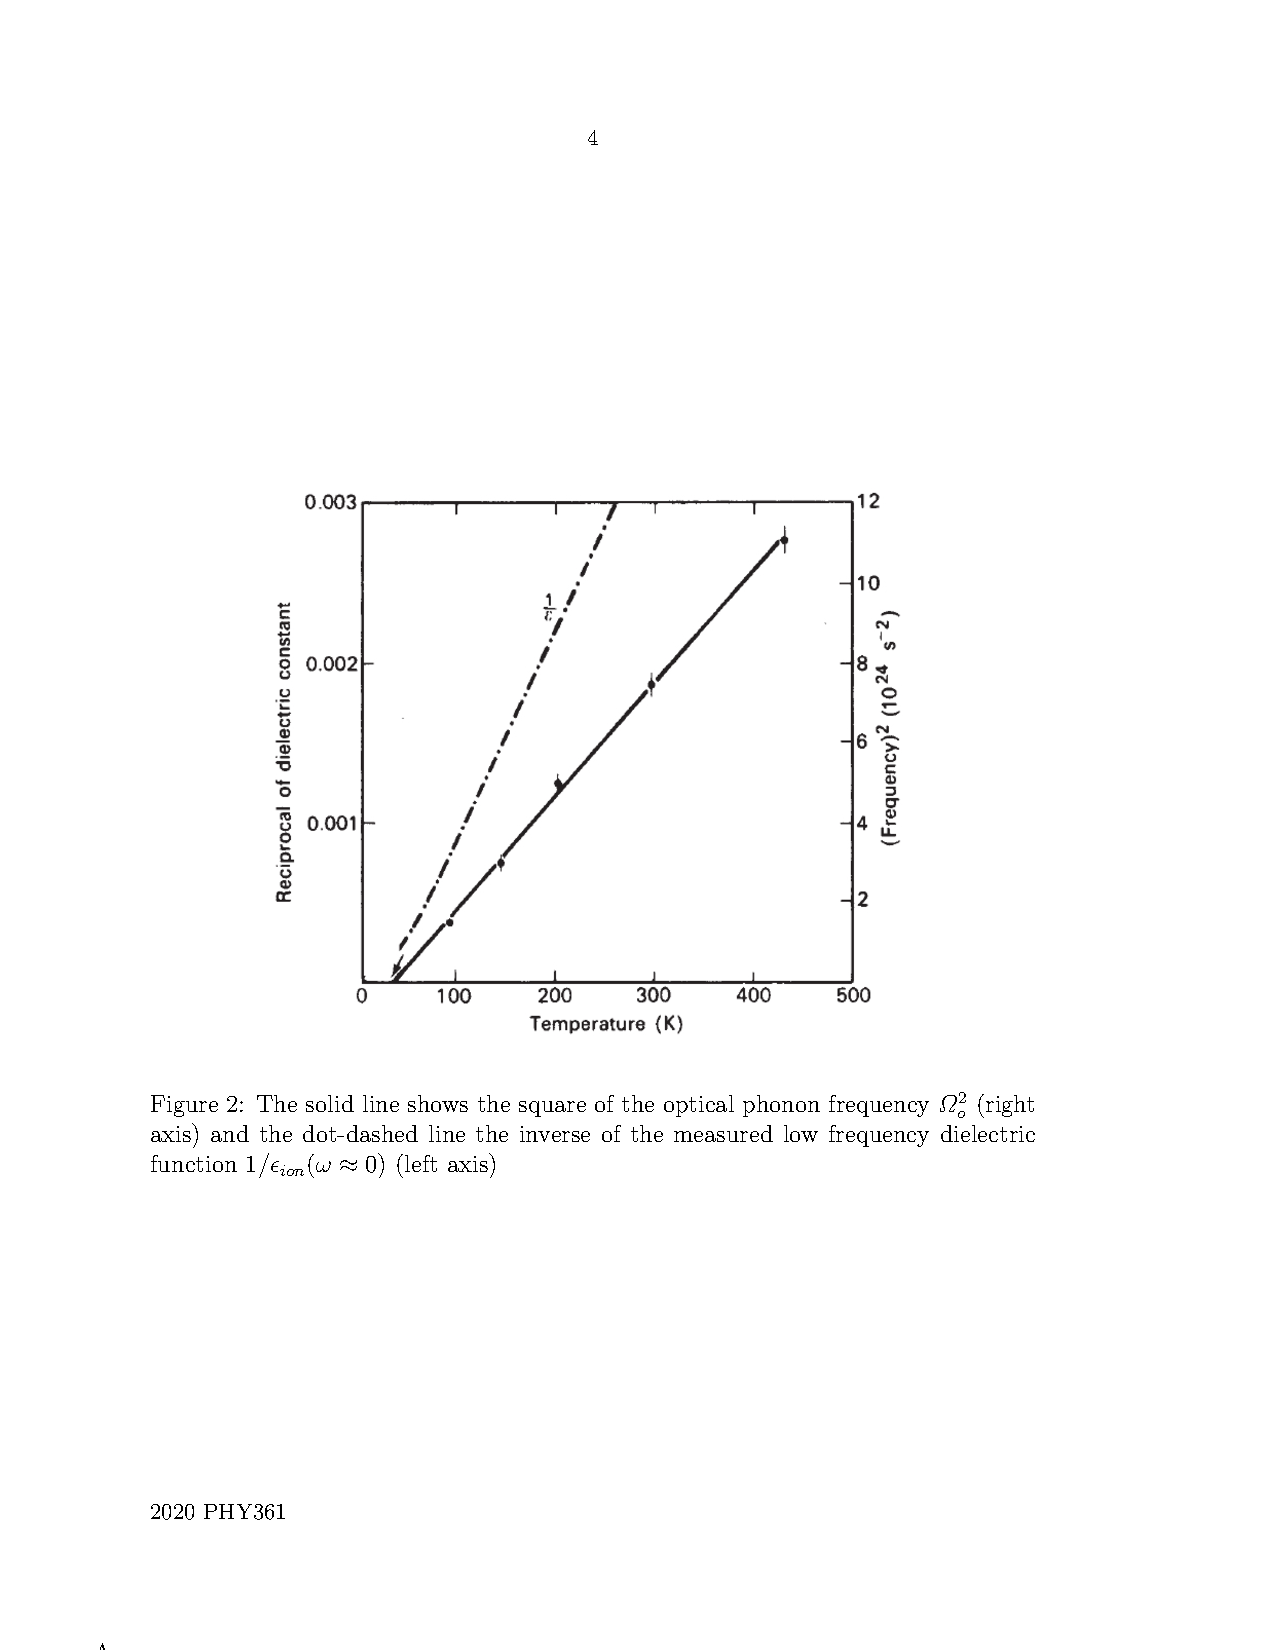
\includegraphics[width=0.5\textwidth,trim=4.5cm 10cm 6cm 8cm,clip]{fig2}
%		\caption{The solid line shows the square of the optical phonon frequency $\Omgo^2$~(right axis) and the dot-dashed line the inverse of the measured low frequency dielectric function $1 / \epsionomgo$~(left axis).}
%		\label{f1}
%	\end{figure}
%}
%
%
%
%\prob{
%	Explain how the extrapolated vanishing of the optical phonon frequency at low temperatures, marked by the arrow in the figure, is indicative of a phase transition.
%}
%
%
%
%\prob{
%	Construct a phenomenological Landau theory for the free energy of the solid as a power series expansion in the polarization, consistent with cubic symmetry.
%}
%
%
%
%\prob{
%	Use your model to predict how the phonon frequency $\Omgo$ and static dielectric constant $\epsion$ would vary with temperature below the critical temperature.
%}

%\makebib

\end{document}
